\documentclass[11pt,a4paper]{amsart}

\usepackage{amsmath,amssymb,amsthm,mathtools}
\usepackage[T1]{fontenc}
\usepackage[utf8]{inputenc}
\usepackage{lmodern}
\usepackage{microtype}
\usepackage[hidelinks]{hyperref}
\hypersetup{
  pdftitle={Synchronized Stress Relative Value: Public-Neutral Option Books under Latent Stress Compression},
  pdfauthor={J. Vidal Llaurado},
  pdfsubject={Synchronization relative value, public-neutral option books, latent stress compression},
  pdfkeywords={option relative value, synchronization risk, Perron stress, public-neutral portfolios, option hedging},
  hypertexnames=false
}
\usepackage{orcidlink}
\usepackage{enumitem}
\usepackage{booktabs}
\usepackage{graphicx}
\usepackage{float}
\usepackage{array}
\usepackage[margin=1in]{geometry}
\raggedbottom

\newcolumntype{L}[1]{>{\raggedright\arraybackslash}p{#1}}
\newcommand{\tablecaptionskip}{\vspace{0.18em}}

\theoremstyle{plain}
\newtheorem{theorem}{Theorem}[section]
\newtheorem{proposition}[theorem]{Proposition}
\newtheorem{lemma}[theorem]{Lemma}
\newtheorem{corollary}[theorem]{Corollary}

\theoremstyle{definition}
\newtheorem{definition}[theorem]{Definition}
\newtheorem{assumption}[theorem]{Assumption}
\newtheorem{condition}[theorem]{Condition}

\theoremstyle{remark}
\newtheorem{remark}[theorem]{Remark}

\DeclareMathOperator{\Var}{Var}
\DeclareMathOperator{\Cov}{Cov}
\DeclareMathOperator{\argmin}{arg\,min}
\DeclareMathOperator{\argmax}{arg\,max}
\DeclareMathOperator{\Span}{span}
\DeclareMathOperator{\diag}{diag}
\newcommand{\R}{\mathbb{R}}
\newcommand{\N}{\mathbb{N}}
\newcommand{\PP}{\mathbb{P}}
\newcommand{\QQ}{\mathbb{Q}}
\newcommand{\EE}{\mathbb{E}}
\newcommand{\cA}{\mathcal{A}}
\newcommand{\cB}{\mathcal{B}}
\newcommand{\cC}{\mathcal{C}}
\newcommand{\cD}{\mathcal{D}}
\newcommand{\cE}{\mathcal{E}}
\newcommand{\cF}{\mathcal{F}}
\newcommand{\cG}{\mathcal{G}}
\newcommand{\cH}{\mathcal{H}}
\newcommand{\cI}{\mathcal{I}}
\newcommand{\cK}{\mathcal{K}}
\newcommand{\cL}{\mathcal{L}}
\newcommand{\cM}{\mathcal{M}}
\newcommand{\cP}{\mathcal{P}}
\newcommand{\cQ}{\mathcal{Q}}
\newcommand{\cR}{\mathcal{R}}
\newcommand{\cS}{\mathcal{S}}
\newcommand{\cT}{\mathcal{T}}
\newcommand{\cU}{\mathcal{U}}
\newcommand{\cV}{\mathcal{V}}
\newcommand{\cX}{\mathcal{X}}
\newcommand{\cZ}{\mathcal{Z}}
\newcommand{\one}{\mathbf{1}}
\newcommand{\dd}{\,d}
\newcommand{\eps}{\varepsilon}
\newcommand{\norm}[1]{\left\lVert #1\right\rVert}
\newcommand{\ip}[2]{\left\langle #1,#2\right\rangle}
\newcommand{\ES}{\operatorname{ES}}

% Preload AMS symbol fonts so microtype expansion is configured before first page use.
\AtBeginDocument{\begingroup\setbox0=\hbox{$\square\mathbb{R}$}\endgroup}

\begin{document}

\title[Synchronized Stress Relative Value]{%
Synchronized Stress Relative Value\\[0.3em]
{\small Public-Neutral Option Books under\\[0.1em] Latent Stress Compression}}
\author[J.~Vidal Llaurad\'o]{J.~Vidal Llaurad\'o\,\orcidlink{0009-0002-1918-5458}}
\thanks{DOI: \href{https://doi.org/10.2139/ssrn.6731781}{10.2139/ssrn.6731781}.}
\email{vidal.llaurado@gmail.com}
\subjclass[2020]{60G22, 91G20, 91G80, 62M15, 62P05}
\keywords{synchronization risk, option relative value, public-neutral portfolios, Perron stress, variance dispersion, incomplete markets, expected shortfall}
\date{May 2026}

\begin{abstract}
Public option calibration can fix a finite public span while leaving synchronized-stress exposure
only partly spanned.  The residual compression is the listed-option relative-value object.  The
trading coordinate is the wedge between index-implied synchronization and an adapted
realized-synchronization benchmark generated by the released Volterra--Perron stress state.  The
sign condition
\[
        \rho^{\mathrm{imp}}_{d,I,\tau}>\widehat\rho^{\mathrm{real}}_{d,I,\tau,w},
\]
selects direction, not size.  Candidate rows are constant-unit listed-option books.  Capital enters
only through the lower-bound sizing equation.  When the index surface embeds more synchronized
stress than admissible single-name variance carriers support, the selected book is short index
convexity and long carrier-basket convexity under public-neutrality, liquidity, cost, and capital
constraints.

Five maps separate the signal, realized benchmark, carrier, book formation, and sizing.  The
implied-synchronization map extracts the coordinate from the index-versus-single-name variance
decomposition.  The realized-synchronization map supplies the released stress-state benchmark.
The carrier map selects single names able to absorb index stress through stress co-movement,
network pressure, relative variance value, and tradability.  The book map selects an element of
the finite listed-option span under public-neutrality constraints and a stress-convexity hedge
ratio.
The sellability map converts the estimated book edge into position size through a lower bound, a
book-risk denominator, and mandate caps.  The main statements identify finite-dimensional
public-neutral optimization, characterize the stress-convexity hedge ratio as the conditional
least-squares projection of index-stress P\&L onto carrier-basket P\&L, prove that the
lower-bound gate certifies positive expected edge under conservative reserves, and separate
adapted lower-bound sizing from future P\&L realization.

The empirical implementation uses listed OptionMetrics contracts, validated underlying prices, and
rolling Oxford--Man Perron stress states.  Over the 2001--2018 execution ledger, the balanced
lower-bound specification forms \(1{,}496\) sign-positive candidate books and allocates capital to
\(906\) rows over \(805\) active dates.  At 1x bid--ask costs it reports total execution P\&L
\(24.567\) million, annualized Sharpe \(3.958\), expected-shortfall loss \(23{,}683\), and max
drawdown \(364{,}148\).  A mechanical leakage audit, cost-stress grid, mandate frontier, dormancy
audit, and capital-realism report accompany the run.  The implementation is formation-adapted
under those checks, but it was developed on the available sample.  The ledger is therefore an
audited sample-developed implementation rather than an unused-sample trading record.
\end{abstract}

\maketitle

\section{Introduction}\label{sec:intro}

Listed index and single-name options supply a finite quote-date span.  They do
not by themselves determine a sellable exposure to latent synchronization.  The synchronization
wedge compares an index-implied synchronization coordinate with an adapted realized-synchronization
benchmark.  The coordinate is finite and mixed-measure; it serves as a relative-value signal rather
than a residual-density selector or recovery theorem.  When the implied coordinate exceeds the
adapted benchmark, the index leg carries excess synchronized-stress convexity relative to the
admissible carrier span.  The selected
book is short index convexity and long carrier convexity.

The wedge inherits its state variable from the market-scale Perron state generated by directed
Volterra contagion \cite{vidal2026market}.  Risk-neutral compression and residual-pricing geometry
supply the public quotient and residual pricing fiber of that state
\cite{vidal2026compression,vidal2026pricing}.  The latent-contagion, dynamic-observability, and
projected-score results provide the physical source-screened input
\cite{vidal2026latent,vidal2026dynamic,vidal2026econometric}.  The finite relative-value book is
the listed-option representative of the resulting synchronization residual.

A synchronization book is admissible only if the carrier side absorbs the prescribed stress
direction.  Relative variance value alone does not turn a basket of single-name straddles into a
synchronization carrier.  The basket must load on the index stress state, lie near the network
stress-transmission direction, carry admissible variance value, and remain in the executable
listed-option span.  The governing object is therefore a book-formation map
\[
        (\text{public surface},\text{latent stress state},\text{listed option span})
        \longmapsto
        \text{admissible synchronization book}.
\]
The map produces a public-neutral book with controlled synchronization-residual exposure and
positive lower-bound sellability, leaving completion of the latent market outside its scope.

The execution problem is finite-dimensional.  Listed options supply a finite span on each quote date.
Delta, vega, gamma, maturity, public-surface principal components, liquidity, bid--ask costs, and
concentration constraints are finite-dimensional controls.  The latent stress geometry enters
through the synchronization wedge, carrier map, danger state, and residual-capital adjustment.
This separates public calibration from listed-option hedgeability.  The Hilbert-space compression
and residual-hedging results in \cite{vidal2026compression,vidal2026pricing} identify the residual
object; the empirical implementation selects a finite listed-contract representative.

The cited literatures enter through different objects.  Option pricing and martingale asset-pricing
theory supply the listed payoff and no-arbitrage background
\cite{blackScholes1973,merton1973,harrisonPliska1981}.  Evidence on option returns, jump premia,
and variance-risk premia supplies the empirical-premium context
\cite{covalShumway2001,bakshiKapadia2003,pan2002,carrWu2009}.  Volatility-surface dynamics,
unspanned volatility, and rough volatility locate the public-surface and span boundaries
\cite{contDaFonseca2002,trolleSchwartz2009,gatheralJaissonRosenbaum2018}.  Incomplete-market and
mean-variance hedging supply the residual-hedge language
\cite{follmerSchweizer1991,schweizer1992meanVariance}.  Good-deal restrictions and
expected-shortfall control enter only at the capital boundary
\cite{cochraneSaaRequejo2000,rockafellarUryasev2000}.

The admitted specification sells excess synchronization only when the carrier side can absorb realized
stress under cost and capital constraints.  The formal sections define the implied
synchronization coordinate, the carrier absorption map, the public-neutral book constraint, the
stress-convexity hedge ratio, the sellability lower bound, the lower-bound sizing projection, and
the capital-risk ledger.

The empirical section implements the sellability map rather than testing full latent recovery.
Candidate books are formed from the sign of the synchronization wedge.  Each source row is a
constant-unit listed-option book, and capital enters only through the lower-bound sizing equation.
The reserve calculation uses entry-known spread, carrier carry, directed-support defects,
danger-state reserves, model-risk reserves, and a pre-formation capital-at-risk denominator.  The
empirical object is a book-level sellability test.  A synchronization wedge is tradable only after
observable cost, carrier, danger, and capital-risk charges are applied before realized P\&L is
observed.

\subsection*{Contributions}

The main object is the lower-bound synchronization book.  Six components define it.

\begin{enumerate}[leftmargin=2em]
\item a synchronization wedge that converts implied-versus-realized correlation information into a
variance-dollar relative-value coordinate;
\item a carrier absorption map that selects the single-name convexity used to protect a short
index-synchronization book;
\item a finite public-neutral option-book optimization with stress-exposure constraints;
\item a stress-convexity hedge ratio that replaces ordinary vega matching by conditional
stress-response matching;
\item a sellability lower bound and lower-bound sizing theorem that separates raw premia from
tradable premia; and
\item an adapted empirical ledger with listed-option execution, adaptedness audit, cost-stress
results, mandate frontier, dormancy audit, and capital-realism accounting.
\end{enumerate}

\subsection*{Organization}

Section~\ref{sec:setup} fixes the filtered listed-option market and the public and latent
information fields.  Section~\ref{sec:sync-wedge} defines the synchronization coordinate and the
variance-dollar wedge.  Section~\ref{sec:carrier} constructs carrier weights.  Section~\ref{sec:book}
defines public-neutral books and proves the finite-dimensional projection and optimization
statements.  Section~\ref{sec:sellability} introduces the lower-bound gate and sizing map.
Section~\ref{sec:capital} records the capital and expected-shortfall ledger.
Section~\ref{sec:empirical} reports the listed-option implementation and empirical audit checks.
Section~\ref{sec:limits} fixes claim boundaries and finite-span extensions.  Section~\ref{sec:conclusion}
returns to the residual sellability boundary.  Appendix~\ref{app:verification} collects the
data-readiness and leakage-audit tables supporting the empirical run.

\section{Listed-option market}\label{sec:setup}

Trading decisions are made on a discrete quote calendar \(d=0,1,\ldots,T\).  The public information
available before trading on date \(d\) is \(\cH_d\).  It contains current and past listed option
quotes, screened public surface summaries, validated underlying prices, and previously released
state estimates.  The latent stress information field is \(\cK_d\), with
\(\cH_d\subseteq\cK_d\).  The latent Perron stress state is a scalar or vector
\[
        P_{d,\mathrm{lat}}^{(w)}\in L^2(\PP,\cK_d),
\]
constructed on rolling windows \(w\in\{63,126,252,504\}\).  The trading rule uses delayed,
latest-available released state estimates
\[
        \widehat P_d^{(w)}\in L^2(\PP,\cH_d).
\]
Every stress-state input used at the date-\(d\) signal-formation time is therefore public at that
formation time.  The released coordinate may estimate a latent \(\cK_d\)-measurable object, but
the execution rule acts only on the \(\cH_d\)-measurable estimate.

Let \(\cU_d\) be the finite set of eligible listed option units on date \(d\).  A unit
\(u\in\cU_d\) is a contract or a small contract package, such as an index straddle or a single-name
straddle in a fixed maturity bucket.  Its next-horizon execution P\&L is denoted
\[
        R_{d,h}(u),
\]
where \(h\) is the holding horizon.  The reported ledger uses weekly holding horizons; one-day and
21-day clocks serve as sensitivity checks.

After the contract basis \(e_u\) is fixed, the executable listed-option span is
\[
        \cS_d:=\Span\{e_u:u\in\cU_d\}\cong\R^{n_d},
        \qquad n_d=|\cU_d|.
\]
A book is a coordinate vector \(x\in\R^{n_d}\) in this span.  Its P\&L is
\[
        R_{d,h}(x)=\sum_{u\in\cU_d}x_u R_{d,h}(u).
\]
The public risk map
\[
        A_d:\R^{n_d}\to\R^{q_d}
\]
collects the public exposures constrained by the book, such as delta, vega, selected
gamma/theta proxies, maturity exposure, index/single-name gross exposure, and public
option-surface principal components.  The vector \(A_d x\) is computed from \(\cH_d\)-measurable
quantities.

\begin{definition}[Public-neutral listed-option book]\label{def:public-neutral-book}
Given a tolerance vector \(\epsilon_d\ge0\), a listed-option book \(x\in\R^{n_d}\) is
\(\epsilon_d\)-public-neutral if
\[
        |A_d x|\le \epsilon_d
\]
coordinatewise.  It is exactly public-neutral if \(\epsilon_d=0\).
\end{definition}

\begin{remark}
Public neutrality is a public-span condition, not absence of latent exposure.  The intended book is
neutral to specified public surface risks while retaining controlled exposure to the synchronization
residual.  This is the trading version of the compression and residual-hedging distinction in
\cite{vidal2026compression,vidal2026pricing}.
\end{remark}

\section{Synchronization wedge}\label{sec:sync-wedge}

The relative-value coordinate must be measured on the scale of the book.  Correlation units
determine sign; variance and premium dollars determine execution.  The map therefore
defines an implied synchronization coordinate and rescales it by the index-versus-single-name
synchronization denominator.

Fix an index \(I\), a maturity bucket \(\tau\), and a state window \(w\).  Let
\[
        c=(I,\tau,w)
\]
denote the cell.  Let \(N_I\) be the admitted constituent universe in the empirical implementation,
and let \(a_{d,i}^{I}\) be the date-\(d\) index weight assigned to name \(i\).  Let
\(\sigma_{d,I,\tau}^{2,\mathrm{imp}}\) be the implied total variance of the index, and let
\(\sigma_{d,i,\tau}^{2,\mathrm{imp}}\) be the implied total variance of name \(i\).  The index
variance decomposition has the schematic form
\[
        \sigma_{d,I,\tau}^{2,\mathrm{imp}}
        =
        \sum_{i\in N_I}(a_{d,i}^{I})^2\sigma_{d,i,\tau}^{2,\mathrm{imp}}
        +
        \rho_{d,c}^{\mathrm{imp}}\,
        \cD_{d,c}^{\mathrm{imp}},
\]
where the synchronization denominator is
\[
        \cD_{d,c}^{\mathrm{imp}}
        =
        2\sum_{i<j}a_{d,i}^{I}a_{d,j}^{I}
        \sigma_{d,i,\tau}^{\mathrm{imp}}
        \sigma_{d,j,\tau}^{\mathrm{imp}}.
\]
Only cells with \(\cD_{d,c}^{\mathrm{imp}}>0\) carry a nondegenerate synchronization denominator.
On those cells, the implied synchronization coordinate is
\[
        \rho_{d,c}^{\mathrm{imp}}
        =
        \frac{
        \sigma_{d,I,\tau}^{2,\mathrm{imp}}
        -
        \sum_{i\in N_I}(a_{d,i}^{I})^2\sigma_{d,i,\tau}^{2,\mathrm{imp}}
        }{
        \cD_{d,c}^{\mathrm{imp}}
        }.
\]
Cells with \(\cD_{d,c}^{\mathrm{imp}}\le0\) are outside this synchronization coordinate unless a
predeclared fallback convention is supplied.

The realized synchronization benchmark is an adapted estimate
\[
        \widehat\rho_{d,c}^{\mathrm{real}}
        =
        \widehat\rho^{\mathrm{real}}(\widehat P_d^{(w)},\text{released directed state}_d,
        \text{realized covariance history}_d),
\]
formed only from information available at signal date \(d\).  The raw synchronization wedge is
\[
        \pi_{d,c}^{\mathrm{sync}}
        =
        \rho_{d,c}^{\mathrm{imp}}-\widehat\rho_{d,c}^{\mathrm{real}}.
\]
Positive values indicate that the option surface prices a larger synchronization component than
the date-\(d\) state-based realized benchmark.  The sign gate is fixed at formation.

The wedge is a mixed-measure trading coordinate.  The coordinate
\(\rho_{d,c}^{\mathrm{imp}}\) is public option-implied, while
\(\widehat\rho_{d,c}^{\mathrm{real}}\) is a \(\PP\)-adapted realized-synchronization benchmark.
The difference is an implied-versus-forecast-realized wedge, not by itself a residual-density
selector or conditional synchronization premium.

\begin{definition}[Variance-dollar synchronization edge]\label{def:sync-edge}
The variance-dollar synchronization edge in cell \(c\) is
\[
        \Delta V_{d,c}^{\mathrm{sync}}
        =
        \pi_{d,c}^{\mathrm{sync}}\,\cD_{d,c}^{\mathrm{imp}}.
\]
Let \(N_{d,c}^{\mathrm{sync}}>0\) be the \(\cH_d\)-measurable conversion from this variance
coordinate to the one-unit listed-option book scale.  It includes the variance notional,
contract multiplier, and book-unit convention used by the implementation.
The cost-adjusted book edge is
\[
        \widehat\mu_{d,c}^{\mathrm{book}}
        =
        N_{d,c}^{\mathrm{sync}}\Delta V_{d,c}^{\mathrm{sync}}
        -\mathrm{TC}_{d,c}
        -\mathrm{Carry}_{d,c}
        -\mathrm{HE}_{d,c}
        -\mathrm{Tail}_{d,c},
\]
where the four subtractions are, respectively, transaction cost, single-name carry drag, hedge
error reserve, and tail-state reserve, all expressed on the same one-unit book scale.
\end{definition}

\begin{remark}
The tradable object is book edge, not raw correlation.  A large
\(\rho^{\mathrm{imp}}-\widehat\rho^{\mathrm{real}}\) is insufficient when the denominator is small,
the carrier is expensive, or the tail reserve is large.  Identifying this finite listed-option
wedge with a dynamic residual premium would require additional projection, basis, and residual
selection assumptions.
\end{remark}

\section{Carrier absorption}\label{sec:carrier}

The long side of a short-synchronization book carries realized index stress when the short index
leg is exposed.  The carrier map selects absorbent convexity, not names by heuristic rank.  It
assigns long convexity to names that co-move with index stress, sit near the network stress
direction, carry admissible variance value, and can be traded at acceptable cost.

For \(i\in N_I\), define the carrier score
\[
        s_{d,c,i}
        =
        z_d\!\left(\beta_{d,c,i}^{\mathrm{stress}}\right)
        +\lambda_1 z_d\!\left(n_{d,w,i}^{\mathrm{net}}\right)
        +\lambda_2 z_d\!\left(v_{d,\tau,i}^{\mathrm{value}}\right)
        -\lambda_3 z_d\!\left(\ell_{d,\tau,i}^{\mathrm{cost}}\right),
\]
where \(z_d\) denotes an adapted cross-sectional normalization.  The terms are
\[
        \beta_{d,c,i}^{\mathrm{stress}}
        =
        \text{train-window response of name \(i\)'s convexity to index stress},
\]
\[
        n_{d,w,i}^{\mathrm{net}}
        =
        \text{network carrier pressure from the rolling latent-state construction},
\]
\[
        v_{d,\tau,i}^{\mathrm{value}}
        =
        \widehat{\mathrm{RV}}_{d,\tau,i}-\mathrm{IVar}_{d,\tau,i}^{\mathrm{imp}},
\]
and \(\ell_{d,\tau,i}^{\mathrm{cost}}\) is a liquidity and bid--ask penalty.  It is taken to be
nonnegative before the adapted cross-sectional normalization is applied.

Raw carrier scores can collapse into a few names.  The shrinkage rule is
\[
        \widetilde s_{d,c,i}
        =
        \omega_{d,c,i}s_{d,c,i}
        +(1-\omega_{d,c,i})
        \left[
        \alpha\,\bar s_{d,c,\mathrm{sector}(i)}
        +(1-\alpha)s_i^{\mathrm{prior}}
        \right],
\]
where \(s_i^{\mathrm{prior}}\) may encode a persistent technology or sector carrier prior, and
\(\omega_{d,c,i}\in[0,1]\) is an adapted reliability weight.

\begin{definition}[Carrier basket]\label{def:carrier-basket}
Let \(p,q>0\), \(\epsilon>0\), and \(\ell_{d,\tau,i}^{\mathrm{cost}}\ge0\).  Assume
\[
        Z_{d,c}^{\mathrm{car}}
        :=
        \sum_{j\in N_I}
        \frac{(\widetilde s_{d,c,j}^{+})^p}
        {(\ell_{d,\tau,j}^{\mathrm{cost}}+\epsilon)^q}
        >0.
\]
If this denominator is zero, the cell is carrier-inadmissible unless a predeclared diversified
fallback basket is supplied.  Otherwise the unconstrained carrier weight is
\[
        \bar b_{d,c,i}
        =
        \frac{(\widetilde s_{d,c,i}^{+})^p/
        (\ell_{d,\tau,i}^{\mathrm{cost}}+\epsilon)^q}
        {Z_{d,c}^{\mathrm{car}}}.
\]
The carrier basket \(b_{d,c}\) is the projection of \(\bar b_{d,c}\) onto the capped simplex
\[
        \Delta_{d,c}
        =
        \left\{
        b\in\R_+^{N_I}:
        \sum_i b_i=1,\quad
        b_i\le b_{\max},\quad
        H(b)\ge H_{\min}
        \right\},
\]
where \(H(b)=-\sum_i b_i\log b_i\) is entropy, with the convention \(0\log0:=0\).
\end{definition}

The carrier projection is a compact finite projection problem.  The proposition identifies the
existence boundary and the convexity condition under which the projection is single-valued.

\begin{proposition}[Existence of carrier weights]\label{prop:carrier-existence}
If \(\Delta_{d,c}\) is nonempty, then a carrier basket \(b_{d,c}\) exists.  If the projection is
taken in squared Euclidean distance, the basket is unique whenever \(\Delta_{d,c}\) is convex.
\end{proposition}

\begin{proof}
The feasible carrier set is a subset of the finite simplex.  The nonnegativity, unit-sum, and cap
constraints are closed and bounded.  Entropy is continuous on the simplex, with the convention
\(0\log0:=0\), so the constraint \(H(b)\ge H_{\min}\) is closed.  Hence \(\Delta_{d,c}\) is compact
whenever it is nonempty.  The squared Euclidean distance from \(\bar b_{d,c}\) is continuous on
\(\Delta_{d,c}\), and the Weierstrass theorem gives existence of a minimizer.

For uniqueness, the nonnegative capped simplex is convex.  Since entropy is concave, its
superlevel set is convex; therefore the displayed \(\Delta_{d,c}\) is convex.  The map
\(b\mapsto \|b-\bar b_{d,c}\|_2^2\) is strictly convex on the ambient Euclidean space and hence on
any affine feasible slice.  A strictly convex objective has at most one minimizer on a convex set.
\end{proof}

\section{Public-neutral synchronization books}\label{sec:book}

Embedding the carrier basket in the listed-option span creates the executable object.  The
primitive book has a short index-convexity leg and a long carrier-convexity leg.  The optimization
then imposes public-risk constraints so that the remaining exposure is the synchronization residual,
not an ordinary surface factor.

Let \(u_I(d,\tau)\) be the selected index convexity unit, for example an index straddle in the
\(\tau\)-day bucket.  Let \(u_i(d,\tau)\) be the corresponding single-name convexity unit.  The
basic short-synchronization book is
\[
        x_{d,c}
        =
        -q_I e_I
        +
        q_B\sum_{i\in N_I}b_{d,c,i}e_i.
\]
The sign convention is that \(q_I>0\) sells index convexity and \(q_B>0\) buys carrier-basket
convexity.

\subsection{Stress-convexity hedge ratio}

The hedge target is stress response, not vega matching.  The book is a synchronization trade, and
the long basket is selected to absorb realized index stress.  Let
\[
        R^I_{d,h}=R_{d,h}(e_I),
        \qquad
        R^B_{d,h}=R_{d,h}\!\left(\sum_i b_{d,c,i}e_i\right).
\]
On a train-window stress set \(\cE_{d,c}^{\mathrm{stress}}\), write
\(\EE_S[\cdot]=\EE_{\mathrm{train}}[\cdot\mid \cE_{d,c}^{\mathrm{stress}}]\).  The conditioning
set is used only when \(\PP_{\mathrm{train}}(\cE_{d,c}^{\mathrm{stress}})>0\).  Define
\[
        \chi_{d,c}
        =
        \frac{
        \Cov_{\mathrm{train}}\!\left(R^I_{d,h},R^B_{d,h}
        \mid \cE_{d,c}^{\mathrm{stress}}\right)
        }{
        \Var_{\mathrm{train}}\!\left(R^B_{d,h}
        \mid \cE_{d,c}^{\mathrm{stress}}\right)+\epsilon
        }.
\]
The book uses \(q_B=\eta_{d,c}\chi_{d,c}^{+}q_I\), with \(0\le\eta_{d,c}\le1\), and then imposes
aggregate gamma and vega bands rather than exact equality.  Cells with \(\chi_{d,c}\le0\) do not have a
positive stress-convexity carrier under this rule.

The coefficient is the stress-conditioned projection of index P\&L onto carrier-basket P\&L.  The
proposition records the least-squares characterization.

\begin{proposition}[Stress-convexity hedge ratio]\label{prop:stress-convexity}
If \(\epsilon=0\) and
\(\Var_{\mathrm{train}}(R^B_{d,h}\mid \cE_{d,c}^{\mathrm{stress}})>0\), then
\(\chi_{d,c}\) is the slope coefficient in the conditional least-squares problem
\[
        \min_{a,\chi\in\R}
        \EE_S\!\left[
        \left(R^I_{d,h}-a-\chi R^B_{d,h}\right)^2
        \right].
\]
Equivalently, it is the no-intercept least-squares coefficient for the centered variables
\(R^I_{d,h}-\EE_S[R^I_{d,h}]\) and \(R^B_{d,h}-\EE_S[R^B_{d,h}]\).
\end{proposition}

\begin{proof}
All moments are taken under the train-window conditional law on
\(\cE_{d,c}^{\mathrm{stress}}\).  Let
\[
        m_I=\EE_S[R^I_{d,h}],
        \qquad
        m_B=\EE_S[R^B_{d,h}].
\]
The conditional loss is a finite quadratic function of \((a,\chi)\).  Differentiation in \(a\)
gives
\[
        a=m_I-\chi m_B.
\]
After substitution the criterion becomes
\[
        \EE_S\!\left[
        \left((R^I_{d,h}-m_I)-\chi(R^B_{d,h}-m_B)\right)^2
        \right].
\]
The first-order condition in \(\chi\) is
\[
        -2\Cov_{\mathrm{train}}(R^I_{d,h},R^B_{d,h}\mid \cE_{d,c}^{\mathrm{stress}})
        +2\chi\Var_{\mathrm{train}}(R^B_{d,h}\mid \cE_{d,c}^{\mathrm{stress}})=0.
\]
The variance assumption removes the null carrier direction and makes the centered quadratic
strictly convex.  The displayed coefficient is therefore the unique least-squares slope.
\end{proof}

\subsection{Finite-dimensional public-neutral optimization}

Let \(\widehat\mu_d\in\R^{n_d}\) be the train-window expected P\&L estimate, let
\(\widehat\Sigma_d\) be a positive semidefinite risk estimate, and let
\(\mathrm{TC}_d(x)\) be a convex transaction-cost penalty.  The book optimization is
\[
        \max_{x\in\R^{n_d}}
        \widehat\mu_d^\top x
        -\lambda x^\top\widehat\Sigma_d x
        -\kappa\mathrm{TC}_d(x)
\]
subject to public-neutrality, gross and net exposure caps, liquidity caps, carrier exposure
constraints, and maturity, ticker, and sector concentration caps.

The theorem states the public-neutral execution problem as a finite constrained optimization.
Existence is compactness.  Uniqueness is strict concavity on the feasible direction span.

\begin{theorem}[Finite public-neutral book optimization]\label{thm:finite-book}
Assume the feasible set \(\cX_d\subset\R^{n_d}\) is nonempty, closed, convex, and bounded, and
assume \(\mathrm{TC}_d\) is convex and lower semicontinuous, with \(\lambda\ge0\) and
\(\kappa\ge0\).  Then the public-neutral book problem has a solution.  If the objective is
strictly concave on \(\cX_d\), for example if \(\lambda>0\) and
\[
        v^\top\widehat\Sigma_d v>0
\]
for every nonzero feasible direction \(v=x-y\) with \(x,y\in\cX_d\), the solution is unique.
\end{theorem}

\begin{proof}
The feasible set is compact by the Heine--Borel theorem.  The linear term and the quadratic risk
term are continuous.  Since \(\mathrm{TC}_d\) is lower semicontinuous and \(\kappa\ge0\), the term
\(-\kappa\mathrm{TC}_d\) is upper semicontinuous.  The full objective is therefore upper
semicontinuous on a compact set, and the Weierstrass theorem gives a maximizer.

For uniqueness, let \(x\ne y\) in \(\cX_d\), set \(v=x-y\), and define
\(z_\theta=\theta x+(1-\theta)y\) for \(0<\theta<1\).  The identity
\[
        z_\theta^\top\widehat\Sigma_d z_\theta
        =
        \theta x^\top\widehat\Sigma_d x
        +(1-\theta)y^\top\widehat\Sigma_d y
        -\theta(1-\theta)v^\top\widehat\Sigma_d v
\]
shows that the quadratic penalty is strictly concave along every nonconstant feasible segment
when the displayed direction condition holds and \(\lambda>0\).  The cost term is concave, and the
return term is affine.  Hence the full objective is strictly concave on \(\cX_d\).  Two distinct
maximizers would make their midpoint feasible and strictly better, which is impossible.
\end{proof}

\begin{remark}
The theorem is a finite listed-option statement.  Infinite-dimensional compression enters only
through the priced stress loading and the residual object.  The executed book is not assumed to
span the full latent market.
\end{remark}

\section{Sellability and lower-bound sizing}\label{sec:sellability}

A synchronization wedge is not automatically sellable.  The lower-bound map separates a raw
coordinate wedge from a wedge that can be traded after costs, model uncertainty, carrier quality,
and tail reserves.  Let \(D_{d,c}\) be an adapted danger score, for example a normalized
combination of Perron level, Perron slope, aggregate realized-volatility acceleration,
directed-contagion breadth, realized synchronization acceleration, and index gap pressure.  The
tail-state reserve in \(\widehat\mu_{d,c}^{\mathrm{book}}\) is part of the one-unit expected
book-edge estimate.  The lower-bound reserve below is an additional conservative haircut applied
when that edge is converted into an admissible capital decision.

\begin{definition}[Sellability lower bound]\label{def:sellability-lb}
For cell \(c\), define
\[
        LB_{d,c}
        =
        \widehat\mu_{d,c}^{\mathrm{book}}
        -z_\alpha\widehat\sigma_{d,c}^{\mathrm{model}}
        -\mathrm{TC}_{d,c}^{\mathrm{round}}
        -\mathrm{Tail}_{d,c}^{\mathrm{reserve}}.
\]
The cell is lower-bound admissible if \(LB_{d,c}>0\).
\end{definition}

The lower bound is a sign certificate, not a complete pricing statement.  The proposition states
the conditional expected-edge claim certified by the reserve inequality.

\begin{proposition}[Lower-bound positive-edge certificate]\label{prop:lb-certificate}
Let \(\EE_d[\cdot]:=\EE[\cdot\mid\cH_d]\).
Suppose the one-period book P\&L \(Y_{d,c}\) satisfies the adapted conservative forecast inequality
\[
        \EE_d[Y_{d,c}]
        \ge
        \widehat\mu_{d,c}^{\mathrm{book}}
        -z_\alpha\widehat\sigma_{d,c}^{\mathrm{model}}
        -\mathrm{TC}_{d,c}^{\mathrm{round}}
        -\mathrm{Tail}_{d,c}^{\mathrm{reserve}}.
\]
If \(LB_{d,c}>0\), then \(\EE_d[Y_{d,c}]>0\).
\end{proposition}

\begin{proof}
By definition of \(LB_{d,c}\), the right-hand side of the forecast inequality is exactly
\(LB_{d,c}\).  Hence \(\EE_d[Y_{d,c}]\ge LB_{d,c}\).  If \(LB_{d,c}>0\), then
\(\EE_d[Y_{d,c}]>0\).
\end{proof}

\begin{definition}[Book-risk denominator]\label{def:book-risk-denominator}
The book-risk denominator \(\mathcal R_{d,c}\) is an \(\cH_d\)-measurable positive reserve for one
unit of the candidate book.  Each input is converted to the same one-unit dollar loss or reserve
scale before the maximum is taken.  In the reported implementation it is the maximum of a settled
pre-formation model-risk reserve, a settled tail-loss reserve, the entry-date spread proxy, a unit
floor, and the formation-date margin proxy:
\[
        \mathcal R_{d,c}
        =
        \max\{
        \widehat\sigma^{\mathrm{hist}}_{d,c},
        \widehat{\ES}^{\mathrm{hist}}_{d,c},
        \mathrm{TC}^{\mathrm{entry}}_{d,c},
        1,
        \mathrm{Margin}^{\mathrm{proxy}}_{d,c}
        \}.
\]
The lower-bound sizing rule uses this one-unit dollar reserve as the quadratic penalty coefficient
for capital allocation.
\end{definition}

\begin{definition}[Lower-bound size]\label{def:lower-bound-size}
Fix a mandate risk-aversion parameter \(\lambda>0\).  The unconstrained lower-bound size is
\[
        x^+_{d,c}
        =
        \frac{(LB_{d,c})_+}{\lambda\mathcal R_{d,c}}.
\]
If \(\bar x^{\mathrm{margin}}_{d,c}\), \(\bar x^{\mathrm{tail}}_{d,c}\), and
\(\bar x^{\mathrm{cost}}_{d,c}\) are the nonnegative \(\cH_d\)-measurable mandate caps generated by
margin, tail-risk, and cost budgets, the executable size is
\[
        x^{\mathrm{exe}}_{d,c}
        =
        \min\left\{
        x^+_{d,c},
        \bar x^{\mathrm{margin}}_{d,c},
        \bar x^{\mathrm{tail}}_{d,c},
        \bar x^{\mathrm{cost}}_{d,c}
        \right\}.
\]
If \(LB_{d,c}\le0\), the executable size is zero.
\end{definition}

The sizing map projects a one-dimensional capital objective onto the nonnegative half-line and the
mandate caps.  The proposition identifies the clipped optimizer.

\begin{proposition}[Lower-bound size as a capital decision]\label{prop:lower-bound-sizing}
For fixed \(\lambda\) and \(\mathcal R_{d,c}>0\), the unconstrained lower-bound size maximizes the
one-dimensional quadratic capital objective
\[
        x\,LB_{d,c}-\frac{\lambda}{2}\mathcal R_{d,c}x^2
        \qquad\text{over }x\ge0.
\]
Applying margin, tail, and cost caps gives the constrained executable size.
\end{proposition}

\begin{proof}
Let
\[
        f(x)=xLB_{d,c}-\frac{\lambda}{2}\mathcal R_{d,c}x^2,
        \qquad x\ge0.
\]
Because \(\lambda>0\) and \(\mathcal R_{d,c}>0\), the function is strictly concave.  Its
first-order condition is
\[
        LB_{d,c}-\lambda\mathcal R_{d,c}x=0.
\]
If \(LB_{d,c}>0\), the unconstrained nonnegative maximizer is
\(LB_{d,c}/(\lambda\mathcal R_{d,c})\); if \(LB_{d,c}\le0\), strict concavity and
\(f'(0)=LB_{d,c}\le0\) put the maximizer at zero.  Thus the unconstrained solution is
\((LB_{d,c})_+/(\lambda\mathcal R_{d,c})\).

The mandate caps reduce the feasible set to the interval
\[
        0\le x\le
        \min\{\bar x^{\mathrm{margin}}_{d,c},
        \bar x^{\mathrm{tail}}_{d,c},
        \bar x^{\mathrm{cost}}_{d,c}\}.
\]
A one-dimensional strictly concave quadratic increases up to its unconstrained maximizer and
decreases after it.  The constrained maximizer is therefore the displayed minimum of the
unconstrained size and the three caps.
\end{proof}

Adaptedness is a measurability statement.  The theorem places the executable vector in the
formation-date information field when the candidate book and sizing inputs are formation-date
measurable.

\begin{theorem}[No-look-ahead lower-bound sizing]\label{thm:no-lookahead}
Let the candidate book, lower bound, book-risk denominator, and mandate caps be
\(\cH_d\)-measurable.  Then the executable lower-bound sized book is \(\cH_d\)-measurable.  In
particular, changing future P\&L, exit prices, future hedging gains, realized exit spreads, or
post-trade costs cannot change the position formed at date \(d\).
\end{theorem}

\begin{proof}
The positive-part map, the reciprocal map on \((0,\infty)\), scalar multiplication by
\(1/\lambda\), and finite minima are Borel measurable.  Hence the map
\[
        (LB,\mathcal R,\text{caps})
        \mapsto
        \min\left\{
        \frac{(LB)_+}{\lambda\mathcal R},
        \bar x^{\mathrm{margin}},
        \bar x^{\mathrm{tail}},
        \bar x^{\mathrm{cost}}
        \right\}
\]
is Borel measurable on the domain \(\mathcal R>0\).  Composition with \(\cH_d\)-measurable inputs
gives an \(\cH_d\)-measurable scalar size.  The candidate book is \(\cH_d\)-measurable by
assumption, and scalar multiplication is a Borel map on the finite listed-option span.  The
executable book is therefore \(\cH_d\)-measurable.  Future P\&L and future cost realizations are
not arguments of the sizing map, so perturbing them cannot change the date-\(d\) position.
\end{proof}

\section{Capital-risk ledger}\label{sec:capital}

The capital ledger maps the mathematical book into quantities observable in the listed-option
execution record.  The reported coordinates are execution P\&L, transaction costs, drawdown,
expected shortfall, gross premium, and margin proxies.  Let \(Y_d\) be daily net execution P\&L and
let
\[
        L_d=(-Y_d)^+
\]
be the daily loss.  The empirical expected-shortfall loss is
\[
        \widehat{\ES}_{95}
        =
        \frac{1}{|\{d:L_d\ge q_{0.95}(L)\}|}
        \sum_{d:L_d\ge q_{0.95}(L)}L_d.
\]
This is the implemented tie convention; if many observations equal the empirical quantile, the
average may include slightly more than the upper five percent of losses.  The max drawdown is
computed from the cumulative P\&L process.  A drawdown budget \(B>0\) is breached if
\[
        \max_t\left(\max_{s\le t}\sum_{u\le s}Y_u-\sum_{u\le t}Y_u\right)>B.
\]

The ledger proposition separates datewise proxy compliance from ex-post drawdown breach.  The
residual breach is the positive part of the excess drawdown.

\begin{proposition}[Capital-budget admissibility]\label{prop:capital-budget}
If the daily book process satisfies the gross-premium, margin, concentration, and drawdown-budget
constraints date by date, then the realized capital ledger is admissible under those proxy
constraints.  If the drawdown budget is breached, the breach amount is exactly
\[
        \max\{\mathrm{MDD}-B,0\}.
\]
\end{proposition}

\begin{proof}
The ledger is a finite collection of proxy coordinates evaluated on the realized book process.  If
the gross-premium, margin, concentration, and drawdown-budget inequalities hold at each admissible
date, the realized ledger remains in the corresponding proxy-admissible set.  Let \(\mathrm{MDD}\)
denote the displayed maximum drawdown.  The drawdown budget is breached exactly on
\(\{\mathrm{MDD}>B\}\).  The excess is \(\mathrm{MDD}-B\) on that event and zero otherwise, hence
\(\max\{\mathrm{MDD}-B,0\}\).
\end{proof}

\begin{remark}
The capital account remains a proxy.  It is closer to deployment than normalized P\&L because it uses
execution dollars, spread costs, gross premium, and margin proxies.  Broker margin, portfolio margin,
financing, borrow, exercise and assignment handling, and hard capacity constraints remain outside
the proxy.
\end{remark}

\section{Listed-option implementation}\label{sec:empirical}

The empirical implementation is a listed-option ledger built from OptionMetrics contracts
\cite{optionMetricsIvydbUs}, validated underlying prices, and rolling Oxford--Man Perron stress
states \cite{lundeShephardSheppard2010}.  Signals are formed from information available at date
\(d\), entered on the next available quote date, and held under predeclared clocks.  The executed
specification is short overpriced synchronization:
\[
        \rho^{\mathrm{imp}}_{d,c}>\widehat\rho^{\mathrm{real}}_{d,c}
        \quad\Rightarrow\quad
        \text{short index convexity plus long carrier-basket convexity,}
\]
subject to the public-neutrality, carrier, cost, and lower-bound constraints above.

\subsection{Data and admissible universe}\label{subsec:data-universe}

The empirical universe is US listed options and US-traded equity underliers.  The option component
uses OptionMetrics contract data for index, liquid ETF, sector ETF, and admitted single-name
candidates; the state component uses Oxford--Man realized-volatility indices to build rolling
physical stress states.  The restriction is empirical, not theoretical.  The definitions above require an index
\(I\), an admissible carrier universe, a finite listed-option span generated by \(\cU_d\), and an
adapted stress state.  The same map can be applied to another option market once those
objects, quote calendars, execution costs, and state inputs are rebuilt.

\begin{table}[H]
\centering
\caption{Data inputs for the empirical implementation.  The execution run is US-option based;
the mathematical map requires an admissible option span, carrier universe, and adapted
stress state.}
\tablecaptionskip
\small
\begin{tabular}{@{}L{0.22\textwidth}L{0.36\textwidth}L{0.35\textwidth}@{}}
\toprule
\textbf{Component} & \textbf{Role in the implementation} & \textbf{Main implementation choices}\\
\midrule
OptionMetrics listed contracts & Tradeable option span, bid--ask execution, Greeks, implied
variance, and straddle/strangle payoffs & US index, ETF, sector ETF, and single-name candidates;
30, 60, and 90 day maturity buckets with liquidity, spread, quote, and maturity filters\\
OptionMetrics forwards and security prices & Forward alignment, underlying close series, and
delta-hedge accounting & Validated ticker-date panel; no delta-hedged execution result is reported
without matched underlying prices\\
Oxford--Man realized-volatility indices & Physical stress state, realized synchronization
benchmark, and aggregate danger controls & Rolling windows \(63,126,252,504\), with \(126\) and
\(252\) as the primary trading windows\\
Directed-contagion state suite & Carrier pressure, directed confirmation, and danger-state
diagnostics & Rolling-only state build with one-day availability and no use of future option
outcomes\\
\bottomrule
\end{tabular}
\label{tab:data-layers}
\end{table}

The data assembly keeps raw contract data, forward alignment, surface-derived coordinates, and
realized-state inputs separate until the trade ledger is formed.  This separation prevents the
exercise from becoming an option-surface fit.  The object is a listed-option execution test of
whether a synchronization wedge remains sellable after carrier, cost, danger-state, and
capital-risk charges.  Appendix~\ref{app:verification} reports the mechanical row counts, leakage
checks, mandate frontier, cost stress, and period audit for the frozen run.

The reported specification is the lower-bound specification defined in Section~\ref{sec:sellability}.  Candidate
books are admitted by the sign-only condition
\[
        \rho^{\mathrm{imp}}_{d,I,\tau}>\widehat\rho^{\mathrm{real}}_{d,I,\tau,w}.
\]
The source rows are constant-unit listed-option books.  The procedure computes the formation-date
synchronization edge, entry-known spread proxy, carrier carry reserve, carrier support reserve,
danger reserve, model-risk reserve, and capital-at-risk denominator.  A row is used only when the
resulting lower bound is positive, and its size is the lower-bound size after mandate margin, tail,
and cost caps.

Four diagnostics bound the evidence.  The dollar execution path records whether the
synchronization book survives listed-option execution and bid--ask costs.  The cost-stress grid
tests sensitivity to spread assumptions.  The mandate frontier locates the selected margin cap
relative to nearby mandate choices.  The adaptedness audit verifies that weights, lower bounds,
and entry-cost proxies are invariant to perturbations of unsettled formation-date and future
realized outcomes.

\begin{remark}[Dormant sellability window]
The lower-bound specification is inactive over part of the mid-2010s.  The latent stress state need
not disappear in that window.  The synchronization wedge can remain present while the
listed-option execution space fails to produce a clean sellability certificate after liquidity,
spread, carrier quality, and capital-risk constraints are imposed.  Raw-exit diagnostics are
consistent with this boundary.  Relaxing the execution gate recovers more trades, but the
additional books are expensive and drawdown-heavy.  The inactivity is therefore a no-trade region
of the public listed-option span.

The market setting of the period gives compatible but non-identifying context.  The 2014--2016
window was a period of compressed US equity volatility, accommodative monetary conditions, calmer
post-crisis risk appetite, and relatively benign realized index stress, although localized stress
episodes still occurred.  The claim is not causal.  The narrower point is that such an environment
can make a positive synchronization wedge less sellable after spread, carrier-quality, and
capital-risk charges.  The absence of trades is then part of the execution certificate rather than
evidence that the latent geometry has vanished.
\end{remark}

Figure~\ref{fig:cumulative-pnl-drawdown} gives the finite ledger diagnostic.  It combines the
return path, drawdown path, annual execution P\&L, execution intensity, and active capital
exposure.  The inactive mid-sample years are visible in the activity and exposure panels.  They are
a no-trade region of the sellability map, not an omitted-data patch.  The rule stands down when the
public listed-option span does not produce an acceptable lower-bound certificate.

\begin{figure}[H]
\centering
\IfFileExists{figures/7-execution-diagnostics.pdf}{%
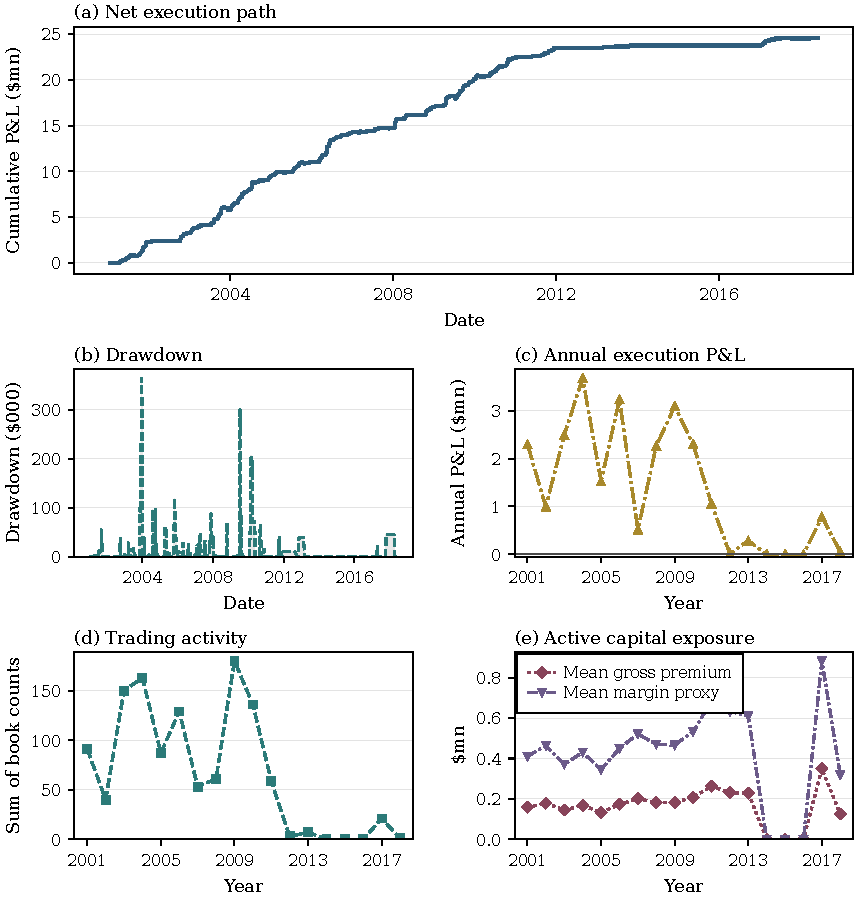
\includegraphics[width=0.98\textwidth]{figures/7-execution-diagnostics.pdf}%
}{%
\fbox{\begin{minipage}[c][0.35\textheight][c]{0.92\textwidth}
\centering
Execution-diagnostics figure unavailable in this source distribution.
\end{minipage}}%
}
\caption{Execution diagnostics at 1x bid--ask costs.  P\&L is delta-hedged listed-option
execution P\&L in dollars.  The panels show cumulative P\&L, drawdown, annual P\&L, trading
activity, and active capital exposure for the lower-bound rule.}
\label{fig:cumulative-pnl-drawdown}
\end{figure}

\begin{table}[t]
\centering
\caption{Lower-bound execution at 1x bid--ask costs.  P\&L is delta-hedged listed-option
execution P\&L in dollars.  Candidate books come from the sign-positive synchronization wedge;
capital is assigned by the lower-bound sizing equation with the formation-date capital-risk
denominator.}
\tablecaptionskip
\small
\begin{tabular}{@{}lrrrrrr@{}}
\toprule
Specification & P\&L & Ann. Sh. & ES95 & Max DD & Active & Used\\
\midrule
Lower-bound & 24.567mn & 3.958 & 23,683 & 364,148 & 805 & 906\\
\bottomrule
\end{tabular}
\label{tab:native-results}
\end{table}

\begin{table}[t]
\centering
\caption{Cost-stress grid for the lower-bound rule.  The same adapted formation weights
are evaluated under higher bid--ask assumptions.  At the 3x bid--ask stress, reported P\&L remains
positive and annualized Sharpe exceeds \(2\); drawdown increases with spread drag.}
\tablecaptionskip
\begin{tabular}{rrrrr}
\toprule
Cost multiplier & P\&L & Ann. Sharpe & ES95 loss & Max drawdown\\
\midrule
0.5 & 28.289mn & 4.187 & 20,197 & 301,264\\
1.0 & 24.567mn & 3.958 & 23,683 & 364,148\\
2.0 & 17.122mn & 3.259 & 31,974 & 501,085\\
3.0 & 9.677mn & 2.107 & 43,306 & 643,465\\
\bottomrule
\end{tabular}
\label{tab:cost-stress}
\end{table}

\begin{table}[t]
\centering
\caption{Capital-realism readout at 1x costs.  Margin quantities are implementation proxies rather
than broker or exchange margin.}
\tablecaptionskip
\begin{tabular}{lr}
\toprule
Quantity & Value\\
\midrule
Total P\&L & 24.567mn\\
Annualized P\&L & 1.414mn\\
Total spread cost & 7.445mn\\
Max margin proxy & 3.493mn\\
Mean active margin proxy & 0.468mn\\
Annualized P\&L / mean active margin & 3.02\\
\bottomrule
\end{tabular}
\label{tab:capital-realism}
\end{table}

\subsection{Adaptedness and uncertainty}

Operational adaptedness is a filtration statement.  At trade formation, the row size uses only
the formation-date synchronization wedge, option and spread information, carrier geometry, danger
variables, mandate caps, and settled pre-formation history.  It does not use future option P\&L,
future delta-hedge P\&L, future returns, exit prices, realized exit-date spreads, future surface
moves, or post-trade realized costs.  The final audit perturbs unsettled formation-date and future
realized P\&L and realized spread columns across \(96\) formation dates.  The maximum change in row
weights, lower bounds, and entry-cost proxies is zero.

The reported Sharpe is bounded by two restrictions.  First, the run is mechanically adapted under
the verification tables in Appendix~\ref{app:verification}.  Second, the architecture was developed
on the available sample.  The run is therefore an audited research implementation rather than a
fresh unused-sample record.  With no unused data available, the evidentiary basis is the sign-only source,
lower-bound sizing, leakage invariance, cost sensitivity, mandate frontier, dormancy audit, capital
realism, and the explicit separation between discovery and execution.

\section{Limitations}\label{sec:limits}

The implementation is recorded mathematically with its boundary conditions fixed.  The empirical
universe is US-centric by design, covering SPX/NDX, US index and sector ETFs, and admitted US
single names.  This keeps the execution span liquid and auditable while leaving the theory outside any
US-equity-specific formulation.  The public-neutral synchronization map is ticker agnostic.  It can be
extended to non-US index options, futures options, country or sector baskets, and other derivative
markets if the listed-option span, carrier universe, public state, and execution-cost model are
rebuilt with the same adaptedness discipline.  A larger \(N\)-universe is the next finite-span
extension.  A broader carrier manifold gives the lower-bound rule more possible synchronized-stress
carriers only while liquidity and execution-cost controls remain binding.

Several objects remain outside the present model.  The risk-neutral pricing component is empirical
rather than a full \(\QQ\)-dynamics for latent Perron stress.  The directed Volterra operator enters
through low-dimensional state summaries rather than a pathwise propagation model.  The payoff space
uses listed-option units and standard Greeks, although the trade is synchronization-based rather
than Black--Scholes-based.  The public-neutrality constraints are finite-dimensional
approximations to the compression and residual-hedging objects in
\cite{vidal2026compression,vidal2026pricing}.  The lower-bound rule is operationally adapted but
sample-developed.

Open extensions are risk-neutral synchronization dynamics, stress-state Greeks, directed Volterra
propagation, and fresh-data or paper-trading evaluation of the lower-bound rule.  The present
result is the finite execution component between latent stress compression and a tradable
synchronization book.

\section{Conclusion}\label{sec:conclusion}

The public-compression and residual-stress geometry of
\cite{vidal2026compression,vidal2026pricing} has a finite listed-option representative.  That
representative is a synchronization book.  Its executable signal is a sign-positive wedge in which
index-implied synchronization exceeds an adapted realized-synchronization benchmark.  The book
sells index convexity against a carrier basket of single-name convexity.  The trade is admitted only
after a lower-bound sellability certificate accounts for spread, carrier support, danger-state
reserves, model-risk reserves, and capital-at-risk.

The empirical implementation reports \(24.567\) million of delta-hedged execution P\&L at 1x
bid--ask costs, with annualized Sharpe \(3.958\), ES95 loss \(23{,}683\), and max drawdown
\(364{,}148\).  These numbers are reported for an audited, sample-developed research
implementation, not a fresh unused-sample trading record.  The mechanical claim is adaptedness.
Formation weights, lower bounds, and entry-cost proxies are invariant to perturbations of future
realized outcomes in the verification audit.

Public option surfaces can leave synchronized stress only partly spanned.  The residual wedge is
not automatically tradable.  It becomes tradable only when the listed-option span supplies an
acceptable carrier and the lower-bound certificate is positive.  Dormancy is therefore part of the
rule's risk discipline.  The book stands down when the public option market does not offer a
sellable synchronization exposure.




\clearpage

\appendix
\setcounter{table}{0}
\renewcommand{\thetable}{A.\arabic{table}}
\renewcommand{\theHtable}{A.\arabic{table}}

\section{Mechanical verification and adaptedness audit}\label{app:verification}

This appendix records the mechanical outputs supporting the empirical section.  The numbers are not
additional tuning criteria.  They are the audit trail for the frozen listed-option implementation.
The tables record the admitted data, constructed windows, lower-bound sizing specification, and
invariance of formation weights to future-outcome perturbations.

\begin{table}[H]
\centering
\caption{Data-readiness summary for the long OptionMetrics/Oxford--Man implementation.  The table
records the admitted contract, underlying, and state inputs before the execution ledger is
evaluated.}
\tablecaptionskip
\begin{tabular}{lll}
\toprule
Object & Check & Value\\
\midrule
Configuration window & First eligible option date & 2000-01-10\\
Configuration window & Last eligible option date & 2018-06-27\\
Core option universe & Option-ready tickers & 32\\
Core underlying panel & Underlying-ready tickers & 32\\
Core underlying panel & Absent underlying rows after validation & 0\\
Option parser & Raw option rows scanned & 74,404,809\\
Option parser & Parsed quote rows & 17,004,261\\
Option parser & Eligible written quotes & 4,951,756\\
Perron state suite & First early-balanced state date & 2000-05-01\\
Perron state suite & State rows across suites & 21,989\\
Directed-contagion suite & State rows across suites & 864,272\\
State windows & Rolling windows & \(63,126,252,504\)\\
\bottomrule
\end{tabular}
\label{tab:app-data-readiness}
\end{table}

\begin{table}[H]
\centering
\caption{Lower-bound execution summary.  Candidate rows are sign-positive synchronization
books; used rows are rows whose lower-bound size remains positive after reserves and mandate
caps.}
\tablecaptionskip
\begin{tabular}{lr}
\toprule
Quantity & Value\\
\midrule
Ledger observations & 1,879\\
Sign-positive candidate books & 1,496\\
Used lower-bound rows & 906\\
Positive lower-bound rows & 906\\
Active dates & 805\\
Total P\&L & 24.567mn\\
Annualized Sharpe & 3.958\\
ES95 loss & 23,683\\
Max drawdown & 364,148\\
Total spread cost & 7.445mn\\
Max margin proxy & 3.493mn\\
\bottomrule
\end{tabular}
\label{tab:app-native-summary}
\end{table}

\begin{table}[H]
\centering
\caption{Adaptedness audit for lower-bound sizing.  The audit perturbs unsettled formation-date
and future realized P\&L and realized spread columns, then recomputes row sizes on audited
formation dates.  The displayed differences are the invariance checks.}
\tablecaptionskip
\begin{tabular}{lr}
\toprule
Audit quantity & Value\\
\midrule
Audited formation dates & 96\\
Maximum weight difference after perturbation & 0\\
Maximum lower-bound difference after perturbation & 0\\
Maximum entry-cost-proxy difference after perturbation & 0\\
Same-day or future realized P\&L used for weight & false\\
Realized exit spread used for weight & false\\
\bottomrule
\end{tabular}
\label{tab:app-leakage-audit}
\end{table}

\begin{table}[H]
\centering
\caption{Mandate frontier for the positive-sync capital-risk specification.  The controls are mandate
inputs rather than signal thresholds.  Here \(\lambda\) is the risk-aversion parameter and the cap
is the daily overlay margin cap.}
\tablecaptionskip
\begin{tabular}{lrrrrr}
\toprule
Profile & \(\lambda\) & Cap & P\&L & Ann. Sharpe & Max DD\\
\midrule
\(0.25,250k\) & 0.25 & 250k & 21.016mn & 3.733 & 363,986\\
\(0.25,500k\) & 0.25 & 500k & 24.567mn & 3.958 & 364,148\\
\(0.25,750k\) & 0.25 & 750k & 25.537mn & 3.978 & 369,585\\
\(0.25,1m\) & 0.25 & 1m & 25.903mn & 3.969 & 369,585\\
\(0.50,750k\) & 0.50 & 750k & 24.708mn & 3.902 & 353,991\\
\(0.50,1m\) & 0.50 & 1m & 25.041mn & 3.891 & 353,991\\
\(1.00,1m\) & 1.00 & 1m & 23.309mn & 3.727 & 347,618\\
\bottomrule
\end{tabular}
\label{tab:app-mandate-frontier}
\end{table}

\begin{table}[H]
\centering
\caption{Cost-stress grid for the balanced lower-bound profile.  Spread costs are stressed after
the same adapted formation weights have been fixed.}
\tablecaptionskip
\begin{tabular}{rrrrr}
\toprule
Cost multiplier & P\&L & Ann. Sharpe & ES95 loss & Max DD\\
\midrule
0.5 & 28.289mn & 4.187 & 20,197 & 301,264\\
1.0 & 24.567mn & 3.958 & 23,683 & 364,148\\
2.0 & 17.122mn & 3.259 & 31,974 & 501,085\\
3.0 & 9.677mn & 2.107 & 43,306 & 643,465\\
\bottomrule
\end{tabular}
\label{tab:app-cost-stress}
\end{table}

\begin{table}[H]
\centering
\caption{Dormancy and raw-exit diagnostics for 2014--2016.  The lower-bound rule stands down in
the eligible panel; looser raw-exit probes recover trades while producing expensive, drawdown-heavy
books.}
\tablecaptionskip
\small
\begin{tabular}{@{}p{0.31\linewidth}rrrrr@{}}
\toprule
Diagnostic & Candidates & Executed & P\&L & Ann. Sh. & Max DD\\
\midrule
Eligible-panel lower-bound specification & -- & 0 & 0 & -- & 0\\
Raw-exit, 10\% spread gate & 304 & 13 & -1.300mn & -0.826 & 1.741mn\\
Raw-exit, 25\% spread gate & 304 & 99 & 1.967mn & 0.366 & 6.048mn\\
\bottomrule
\end{tabular}
\label{tab:app-dormancy}
\end{table}

\clearpage

\bibliographystyle{unsrt}
\bibliography{references}

\end{document}
